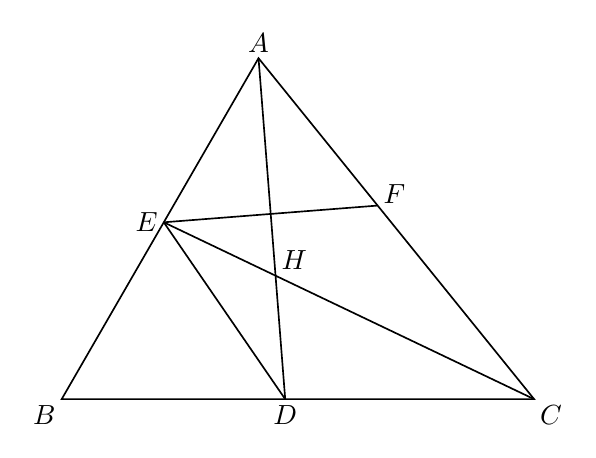
\begin{tikzpicture}[x=1cm,y=1cm,font=\normalsize,
 geometry edge/.style={solid,line width=.6pt},
 geometry mark/.style={solid,line width=.6pt},
 geometry label/.style={font=\normalsize,inner sep=2pt}]
\coordinate (A) at (2.5,4.3301);
\coordinate (B) at (0.0,0.0);
\coordinate (C) at (6.0,0.0);
\coordinate (D) at (2.8388,0.0);
\coordinate (E) at (1.2967,2.246);
\coordinate (F) at (4.0128,2.4585);
\coordinate (H) at (2.7161,1.5682);
\draw[geometry edge] (A)--(E)--(B)--(D)--(C)--(F)--cycle;
\draw[geometry edge] (A)--(H)--(D);
\draw[geometry edge] (E)--(H)--(C);
\draw[geometry edge] (E)--(D);
\draw[geometry edge] (E)--(F);
\node[geometry label,above] at (A) {$A$};
\node[geometry label,below left] at (B) {$B$};
\node[geometry label,below right] at (C) {$C$};
\node[geometry label,below] at (D) {$D$};
\node[geometry label,left] at (E) {$E$};
\node[geometry label,right,yshift=4pt] at (F) {$F$};
\node[geometry label,above right] at (H) {$H$};
\end{tikzpicture}
